%=====================================================================
\section[Quantum zero-point motion and quantum melting]{Quantum kinetic energy, zero-point motion and quantum melting}\label{qm:sec}

Everything so far in this chapter, and everything in Chapters~1--3, is classical: particles sit at points, and at
zero temperature they sit \emph{still}, at a minimum of the energy. Quantum mechanics forbids this. A particle confined
to a region of size $L$ has momentum uncertainty of order $\hbar/L$ and therefore a kinetic energy of order
$\hbar^2/(mL^2)$, even at $T=0$. A crystal of light particles may not exist at all, however favourable the potential
energy of the triangular arrangement: the zero-point motion can melt it. This section asks when that happens. It
uses the two-dimensional electron crystal (Riesz $s=1$ with a background, Section~\ref{sec:ch4-plasmas} and
Section~\ref{sec:num-jellium}) as its worked example, and ends with a newer family of systems, electrons and excitons
in transition-metal dichalcogenides (TMDs).

\begin{warnbox}[: the theorem is classical]
The theorem of Chapter~2 compares \emph{classical} energies of \emph{point configurations}. A quantum crystal is a
many-body wave function, and its energy contains kinetic terms that no point configuration has. Nothing in this
section is a consequence of the theorem, and nothing in it is Tier~A. What the theorem does supply is the starting
point of the quantum calculation: the classical arrangement around which the particles vibrate. Where that
arrangement is the triangular lattice, the theorem (for potentials in its class) or the jellium result of
Chapter~5 (Tier~L, for $s=1$) tells us so; the vibrations themselves are physics, \tierC{} when we derive them and
\tierX{} when we compute them.
\end{warnbox}

%---------------------------------------------------------------------
\subsection{Scaling: kinetic against potential energy}\label{qm:sec-scaling}

Take particles of mass $m$ in the plane, at area density $n$, with pair potential $V(r)=C/r^s$ ($C>0$). Two
energies compete.
\begin{itemize}
\item \emph{Potential energy per particle.} The typical spacing is $\ell=n^{-1/2}$, so the potential energy per
particle is of order $C\ell^{-s}=C\,n^{s/2}$. For $s>2$ the lattice sum converges and this is exact up to a
constant: Chapter~2's \lean{riesz_lattice_homogeneous} says the lattice energy at density $\rho$ is $\rho^{s/2}$ times
its value at density one \tierA. For $s\le2$ only the background-subtracted (jellium) energy is finite, and it scales
the same way.
\item \emph{Kinetic energy per particle.} If each particle is localised in its own cell, of area $1/n$, the
uncertainty principle gives momenta of order $\hbar\sqrt n$ and a kinetic energy of order $\hbar^2 n/m$. If instead
the particles form a Fermi liquid, the kinetic energy is the Fermi energy, which in two dimensions is also
proportional to $\hbar^2n/m$ (Exercise~\ref{qm:ex-fermi}).
\end{itemize}
The ratio of the two is therefore
\begin{equation}\label{qm:eq-ratio}
\frac{\text{potential}}{\text{kinetic}}\;\sim\;\frac{C\,n^{s/2}}{\hbar^2n/m}\;=\;\frac{mC}{\hbar^2}\;n^{(s-2)/2}
\end{equation}
\tierC{} (a dimensional argument; all numerical factors are dropped). A crystal needs the potential energy to win.
The exponent $(s-2)/2$ decides \emph{where}:
\begin{itemize}
\item $s<2$, including the Coulomb law $s=1$: the ratio grows as $n\to0$. Quantum crystals form at \emph{low}
density. This is Wigner's original picture of electrons.
\item $s>2$, for example dipoles, $s=3$: the ratio grows as $n\to\infty$. Quantum crystals form at \emph{high}
density, and dilute systems are quantum fluids.
\item $s=2$: the ratio $mC/\hbar^2$ does not depend on the density at all. The inverse-square law and the kinetic
energy scale identically under dilation, so the density cannot tip the balance; only the coupling constant can.
\end{itemize}

\begin{remark}[two different $s=2$ endpoints]\label{qm:rem-s2}
Chapter~5 (the subsection on the endpoint $s=2$ and Remark~\ref{ch5:rem:s2}) explains why $s=2$ is the endpoint of the
\emph{classical} theory in the plane: there $s=d$, the interaction $|x|^{-2}$ is not locally integrable, and the
jellium energy is undefined. The quantum marginality above is a different statement: the kinetic energy scales like
$L^{-2}$ in \emph{every} dimension, so $s=2$ is quantum-marginal in any $d$. The two endpoints coincide only because
$d=2$. They are two obstructions that happen to sit at the same exponent in the plane, not one obstruction seen
twice \tierC.
\end{remark}

\paragraph{The density parameter $r_s$.} For electrons ($C=e^2$, where here and below $e^2$ stands for
$e^2/4\pi\varepsilon_0$, the Coulomb convention of Section~\ref{sec:ch4-plasmas}) the natural length is the Bohr
radius $a_B=\hbar^2/(me^2)$, and the natural energy is the Hartree $e^2/a_B$. Define the \emph{Wigner--Seitz radius}
$a_{\rm ws}$ by
\begin{equation}\label{qm:eq-rs}
\pi a_{\rm ws}^2\,n = 1,\qquad r_s=\frac{a_{\rm ws}}{a_B}.
\end{equation}
A disk of radius $a_{\rm ws}$ contains one electron on average. With $C=e^2$, $s=1$, \eqref{qm:eq-ratio} reads
$(me^2/\hbar^2)\,n^{-1/2}=\sqrt\pi\,r_s$: \emph{$r_s$ is the potential-to-kinetic ratio}, and large $r_s$ means low
density and a crystal. In the triangular lattice of density $n$ the cell area is $\frac{\sqrt3}{2}a^2=1/n$, so the
nearest-neighbour spacing is
\begin{equation}\label{qm:eq-a}
a=\Bigl(\frac{2\pi}{\sqrt3}\Bigr)^{1/2}a_{\rm ws}=1.904626\,a_{\rm ws}.
\end{equation}
We will need both lengths, and we will say each time which one is meant.

%---------------------------------------------------------------------
\subsection{Harmonic phonons of the Wigner crystal}\label{qm:sec-phonons}

Let the electrons sit at the triangular sites $R$ and displace each by a small $u_R$. Expanding the jellium energy to
second order (the first order vanishes because every site is a centre of symmetry) gives
\[
E=E_0+\frac14\sum_{R\ne R'}(u_R-u_{R'})^{\!\top}\,\Phi(R-R')\,(u_R-u_{R'})+O(u^3),
\]
where $\Phi(x)$ is the $2\times2$ Hessian of $e^2/|x|$ in the plane. The uniform background contributes nothing at this
order: the potential of an infinite uniform sheet is the same at every point of the sheet, so it exerts no in-plane
force \tierC. For a radial function $f(r)$, $\Phi=f''\,\hat x\hat x^{\top}+\frac{f'}{r}(I-\hat x\hat x^\top)$; for $f=e^2/r$
this is $e^2r^{-3}(2\hat x\hat x^\top-(I-\hat x\hat x^\top))$: stiff along the bond, soft (negative) across it, with
trace $e^2/r^3$. Newton's equations $m\ddot u_R=-\sum_{R'}\Phi(R-R')(u_R-u_{R'})$ with $u_R=\varepsilon\,e^{\mathrm
i(k\cdot R-\omega t)}$ give the eigenvalue problem $\omega^2\varepsilon=D(k)\varepsilon$ with the \emph{dynamical
matrix}
\begin{equation}\label{qm:eq-D}
D(k)=\frac1m\sum_{R\ne0}\Phi(R)\,\bigl(1-\cos k\cdot R\bigr)=\Psi(0)-\Psi(k),\qquad
\Psi(k)=\frac1m\sum_{R\ne0}\Phi(R)\cos k\cdot R .
\end{equation}
Its two eigenvalues are the squared frequencies $\omega_T^2(k)\le\omega_L^2(k)$ of the transverse and longitudinal
branches. Since $|\Phi(R)|\sim R^{-3}$ the sums converge absolutely in the plane, but slowly, and the interesting
long-wavelength behaviour comes from the far tail. Bonsall and Maradudin computed this spectrum by Ewald's
method~\cite{bm} \tierL; we do the same, following the energy derivation of Proposition~\ref{prop:ewald}.

\begin{proposition}[Ewald form of $\Psi$]\label{qm:prop-ewald}
Split $1/r=\operatorname{erfc}(\alpha r)/r+\operatorname{erf}(\alpha r)/r$ and let $\Phi_S$ be the Hessian of the
first part. In units $e=m=1$, with cell area $A_c=1/n$ and reciprocal lattice vectors $G$,
\begin{equation}\label{qm:eq-psi-ewald}
\Psi(k)=\sum_{R\ne0}\Phi_S(R)\cos k\cdot R\;-\;\frac1{A_c}\sum_{G,\ G\ne k}\frac{2\pi}{|G-k|}
\operatorname{erfc}\Bigl(\frac{|G-k|}{2\alpha}\Bigr)(G-k)(G-k)^{\!\top}\;+\;\frac{4\alpha^3}{3\sqrt\pi}\,I ,
\end{equation}
and the result does not depend on $\alpha$.
\end{proposition}
\begin{humanproof}
\tierC{} (a sketch in the style of Proposition~\ref{prop:ewald}). Let $T(x)=\sum_R e^{\mathrm ik\cdot R}\,
\frac{\operatorname{erf}(\alpha|R-x|)}{|R-x|}$, a smooth function of $x$. Its Hessian at $x=0$ is
$\sum_R e^{\mathrm ik\cdot R}\Phi_L(R)$, including the term $R=0$. Poisson summation, with the two-dimensional Fourier
transform $\frac{2\pi}{q}\operatorname{erfc}(\frac q{2\alpha})$ of $\operatorname{erf}(\alpha r)/r$, turns $T(x)$
into $\frac1{A_c}\sum_G e^{-\mathrm i(G-k)\cdot x}\,\frac{2\pi}{|G-k|}\operatorname{erfc}\bigl(\frac{|G-k|}{2\alpha}\bigr)$,
whose Hessian at $x=0$ is the middle term of \eqref{qm:eq-psi-ewald}. The Taylor expansion
$\operatorname{erf}(\alpha r)/r=\frac{2}{\sqrt\pi}(\alpha-\frac{\alpha^3r^2}3+\dots)$ shows that the $R=0$ term is
$\Phi_L(0)=-\frac{4\alpha^3}{3\sqrt\pi}I$; subtracting it gives the last term. The imaginary parts cancel because the
lattice is symmetric under $R\mapsto-R$.
\end{humanproof}

\paragraph{The $G=0$ term and the plasmon.} In \eqref{qm:eq-psi-ewald} the reciprocal vector $G=0$ contributes the
term with $q=G-k=-k$. At $k=0$ it is absent ($q\,q^\top\cdot 2\pi/|q|\to0$); this is where the background acts, as
in the energy. At $k\ne0$ it is \emph{present}, and it is the most important term at long wavelength: it adds
$\frac{2\pi n e^2}{m}\,|k|\,\hat k\hat k^\top$ to $D(k)$, so the longitudinal branch is a two-dimensional plasmon,
\begin{equation}\label{qm:eq-plasmon}
\omega_L^2(k)\simeq\frac{2\pi n e^2}{m}\,|k|\qquad(k\to0),
\end{equation}
while the transverse branch is an ordinary sound wave, $\omega_T\simeq c_T|k|$ \tierC. Dropping the $q=-k$ term at
$k\ne0$ (``the background cancels $G=0$'') is a natural mistake. It is our negative control below.

\paragraph{Reduced units.} Measure lengths in $a_{\rm ws}$ and frequencies in $(e^2/ma_{\rm ws}^3)^{1/2}$. Then
$A_c=\pi$, $n=1/\pi$, \eqref{qm:eq-plasmon} becomes $\omega_L^2\simeq2|k|$, and all the physics of the density is in
one conversion factor: in Hartree atomic units ($\hbar=m=e^2=1$, $a_{\rm ws}=r_s$),
\begin{equation}\label{qm:eq-omega-units}
\hbar\,\omega_{\rm phys}=\omega_{\rm red}\;r_s^{-3/2}\ \text{Hartree}.
\end{equation}

%---------------------------------------------------------------------
\subsection{Zero-point energy and zero-point displacement}\label{qm:sec-zp}

Each normal mode $(k,\lambda)$ is a harmonic oscillator. In its ground state it has energy $\frac12\hbar\omega_\lambda(k)$
and contributes $\hbar/(2m\omega_\lambda(k))$ to the mean square displacement of a particle (sum of both Cartesian
components, divided among the $N$ particles). For a crystal of $N$ particles with periodic boundary conditions the $k$
run over $N$ points of the Brillouin zone (BZ), and as $N\to\infty$ the sums become BZ averages
$\langle\cdot\rangle_{\rm BZ}$:
\begin{equation}\label{qm:eq-zp}
E_{\rm zp}=\frac{\hbar}{2}\Bigl\langle\sum_\lambda\omega_\lambda\Bigr\rangle_{\rm BZ},\qquad
\langle|u|^2\rangle_{T=0}=\frac{\hbar}{2m}\Bigl\langle\sum_\lambda\frac1{\omega_\lambda}\Bigr\rangle_{\rm BZ}.
\end{equation}

\begin{proposition}[the zero-point displacement is finite in two dimensions]\label{qm:prop-finite}
With $\omega_L^2\simeq2\pi ne^2|k|/m$ and $\omega_T\simeq c_T|k|$ near $k=0$, both BZ averages in \eqref{qm:eq-zp}
are finite. The classical mean square displacement at temperature $T>0$,
$\langle|u|^2\rangle_T=\frac{k_BT}{m}\langle\sum_\lambda\omega_\lambda^{-2}\rangle_{\rm BZ}$, is infinite: on a
crystal of $N$ particles it grows like $\frac{k_BT}{4\pi n m c_T^2}\ln N$.
\end{proposition}
\begin{humanproof}
\tierC. Only the neighbourhood of $k=0$ can cause trouble, provided the frequencies are positive elsewhere (our
numerics find no imaginary frequency on any grid used, \tierX). In polar
coordinates $d^2k=|k|\,d|k|\,d\theta$. Then $\int_0 \frac{|k|\,d|k|}{c_T|k|}$ and
$\int_0\frac{|k|\,d|k|}{|k|^{1/2}}$ converge, but $\int_0\frac{|k|\,d|k|}{c_T^2|k|^2}=\frac1{c_T^2}\int_0\frac{d|k|}{|k|}$
diverges logarithmically. On a crystal of $N=L^2n$ particles the smallest wave number is of order $1/L$, so the
divergent integral is cut off at $|k|\sim N^{-1/2}$. The BZ has area $(2\pi)^2n$, and the average of
$c_T^{-2}|k|^{-2}$ over it, cut off below at $k_{\min}$, is $\frac{2\pi}{(2\pi)^2n\,c_T^2}\ln\frac1{k_{\min}}+O(1)$,
which is $\frac{1}{4\pi n c_T^2}\ln N+O(1)$. The longitudinal branch adds a finite amount.
\end{humanproof}

The second half is the harmonic version of the Mermin--Wagner--Peierls phenomenon: a two-dimensional crystal at
$T>0$ has no true long-range positional order, because the displacement of a particle relative to a distant one
grows without bound~\cite{mermin} \tierL. The first half is why the \emph{quantum} problem is well posed: at $T=0$ the
displacement of a single particle is finite.

\paragraph{The $r_s$ laws.} By \eqref{qm:eq-omega-units} and \eqref{qm:eq-zp}, in Hartree atomic units,
\begin{equation}\label{qm:eq-laws}
E_{\rm zp}=c_{\rm zp}\,r_s^{-3/2}\ \text{Ha},\quad c_{\rm zp}=\tfrac12\bigl\langle\textstyle\sum_\lambda\omega_{\rm
red}\bigr\rangle;\qquad
\frac{\langle|u|^2\rangle}{a_{\rm ws}^2}=\frac{\tfrac12\langle\sum_\lambda\omega_{\rm red}^{-1}\rangle\,r_s^{3/2}}{r_s^2}
=C_{\rm ws}\,r_s^{-1/2} .
\end{equation}
The displacement grows like $r_s^{3/4}$ (in bohr) but the spacing grows faster, like $r_s$; the \emph{relative}
zero-point motion $\langle|u|^2\rangle^{1/2}/a$ therefore decreases like $r_s^{-1/4}$. Dilute electrons are \emph{more}
classical, as the scaling of \S\ref{qm:sec-scaling} said. With \eqref{qm:eq-a},
\begin{equation}\label{qm:eq-C}
\gamma^2:=\frac{\langle|u|^2\rangle}{a^2}=C\,r_s^{-1/2},\qquad C=\frac{C_{\rm ws}}{2\pi/\sqrt3}.
\end{equation}

\paragraph{The computation.} The script \texttt{code/quantum\_melting.py} (numpy and scipy only; sympy and mpmath
for the last check) evaluates \eqref{qm:eq-psi-ewald}, diagonalises $D(k)$, and averages over half-shifted
(Monkhorst--Pack) $m\times m$ grids of the reciprocal cell, which never contain $k=0$ (function \texttt{mp\_grid}). The core is:
\lstinputlisting[language=Python,firstline=34,lastline=63,caption={\texttt{code/quantum\_melting.py}, lines 34--63
(verbatim, read from the file at compile time).}]{code/quantum_melting.py}

Before any number is read, the script runs three positive controls: (P1) the $\alpha$-independence of $D(k)$;
(P2) the trace sum rule $\operatorname{tr}D(k)=\sum_{R\ne0}(1-\cos k\cdot R)/R^3$, evaluated \emph{without} Ewald by a
direct sum over $|R|\le400$ plus the tail $2\pi/(A_c\cdot400)$; (P3) the plasmon limit \eqref{qm:eq-plasmon}. Then it
computes the BZ averages, the literature comparison, and two negative controls: (N1) the classical displacement of
Proposition~\ref{qm:prop-finite}, which must grow like $\ln m$ with the predicted slope; (N2) the same calculation
with the $q=-k$ term dropped at $k\ne0$.

\begin{numbox}[: output of \texttt{quantum\_melting.py} (Tier X)]
Command, exactly as run (two cores, 32\,s wall time):
\begin{lstlisting}
taskset -c 6,7 /home/callensxavier_gmail_com/AutoevolveAI/.venv/bin/python -I /home/callensxavier_gmail_com/AutoevolveAI/.claude/worktrees/openai-math-discovery/papers/textbook_universal_optimality/code/quantum_melting.py /home/callensxavier_gmail_com/AutoevolveAI/.claude/worktrees/openai-math-discovery/papers/textbook_universal_optimality/figures_v2/qm_phonons_lindemann.pdf
\end{lstlisting}
Output, verbatim:
\begin{lstlisting}
== P1 Ewald alpha-invariance of D(k) at 5 random k (max |D_a - D_1|)
   alpha=0.6: 7.77e-16
   alpha=1.6: 1.55e-15
== P2 trace sum rule: tr D(k) vs direct sum_{R!=0} (1-cos k.R)/R^3 (R<=400, tail 2pi/(A_c Rmax))
   k=(+0.250,+0.794): Ewald 1.285203  direct 1.285203
   k=(+0.551,-0.550): Ewald 1.224116  direct 1.224116
   k=(-0.400,+0.747): Ewald 1.300996  direct 1.300997
== P3 long-wavelength limits along Gamma-M (expect omega_L^2/k -> 2 pi n = 2)
   k=1e-02: omega_L^2/k = 1.993087   omega_T/k = 0.371833
   k=1e-03: omega_L^2/k = 1.999309   omega_T/k = 0.371837
   k=1e-04: omega_L^2/k = 1.999931   omega_T/k = 0.371837
== zero-point quantities on m x m Monkhorst-Pack grids (reduced units)
    m   <sum w>        <sum 1/w>      <sum 1/w^2>
    12  1.6276631027  3.5780591325  12.91144858
    24  1.6274214829  3.6212846016  15.42657855
    48  1.6273804394  3.6425288246  17.93709045
    96  1.6273733348  3.6530563524  20.44564306
   192  1.6273720970  3.6582900165  22.95323582
   384  1.6273718805  3.6608965985  25.46035918
   observed orders: <sum w> p=2.52, <sum 1/w> p=1.01; Richardson: 1.62737183, 3.66348284
RESULT c_zp = 0.813686 Ha = 1.627372 Ry   (E_zp = c_zp r_s^-3/2); literature 0.814 Ha [BM via DN]: rel diff -3.86e-04
RESULT <|u|^2> = 1.831741 a_ws^2 r_s^-1/2 ;  <|u|^2>/a^2 = C r_s^-1/2 with C = 0.504946  (a/a_ws = 1.904626)
== N1 classical <|u|^2> at T>0 is proportional to <sum 1/w^2>: grows like log m (Mermin-Wagner)
   slope d<sum 1/w^2>/d ln m (m 192->384) = 3.61701; predicted 1/(2 c_T^2) = 3.61630
== N2 dropping the G = 0 reciprocal term at k != 0 (wrong background handling), 48 x 48 grid
   fraction of k with an imaginary branch (omega^2<0): 0.064;  min omega^2 -0.0417
   at k=1e-3 along Gamma-M: omega^2 = 1.383e-07, 4.371e-07 (no sqrt(k) plasmon)
== Lindemann: gamma^2 = <|u|^2>/a^2 = C r_s^-1/2  =>  r_s* = (C/gamma_c^2)^2
   gamma_c=0.20: r_s* =    159.4
   gamma_c=0.22: r_s* =    108.8
   gamma_c=0.24: r_s* =     76.9
   gamma_c=0.26: r_s* =     55.8
   gamma_c=0.28: r_s* =     41.5
   gamma_c=0.30: r_s* =     31.5
   gamma_c=0.33: r_s* =     21.5
   gamma_c=0.36: r_s* =     15.2
   gamma_c=0.40: r_s* =     10.0
   harmonic gamma at r_s=31.0: 0.3011
   harmonic gamma at r_s=37.0: 0.2881
== Relative (nearest-neighbour) displacement, delta = a1: finite at T > 0, unlike <|u|^2>
    m   classical <sum (1-cos k.delta)/w^2>   quantum <sum (1-cos k.delta)/w>
    48  5.40267931                        2.85595420
    96  5.40180638                        2.85594433
   192  5.40158898                        2.85594311
   384  5.40153469                        2.85594296
   classical gamma_rel^2 = <|u_i-u_j|^2>/a^2 = (2/Gamma) * 5.401535 / (a/a_ws)^2 = 2.978022/Gamma; at Gamma = 137: gamma_rel = 0.1474
   quantum (T=0) gamma_rel^2 = 0.787282 r_s^-1/2; at r_s = 31: gamma_rel = 0.3760
== Exciton potential h(t) = 2/sqrt(t) - 2/sqrt(t + d^2), t = r^2: signs of (-1)^r h^(r), r = 0..10
   exciton d^2=1/10      :   0 negative values out of 275; first failure (r, t) = None
   exciton d^2=1         :   0 negative values out of 275; first failure (r, t) = None
   exciton d^2=10        :   0 negative values out of 275; first failure (r, t) = None
   control Lennard-Jones : 123 negative values out of 275; first failure (r, t) = (0, 1.7782794100389228)
figure written: /home/callensxavier_gmail_com/AutoevolveAI/.claude/worktrees/openai-math-discovery/papers/textbook_universal_optimality/figures_v2/qm_phonons_lindemann.pdf
\end{lstlisting}
\end{numbox}

\begin{figure}[t]
\centering
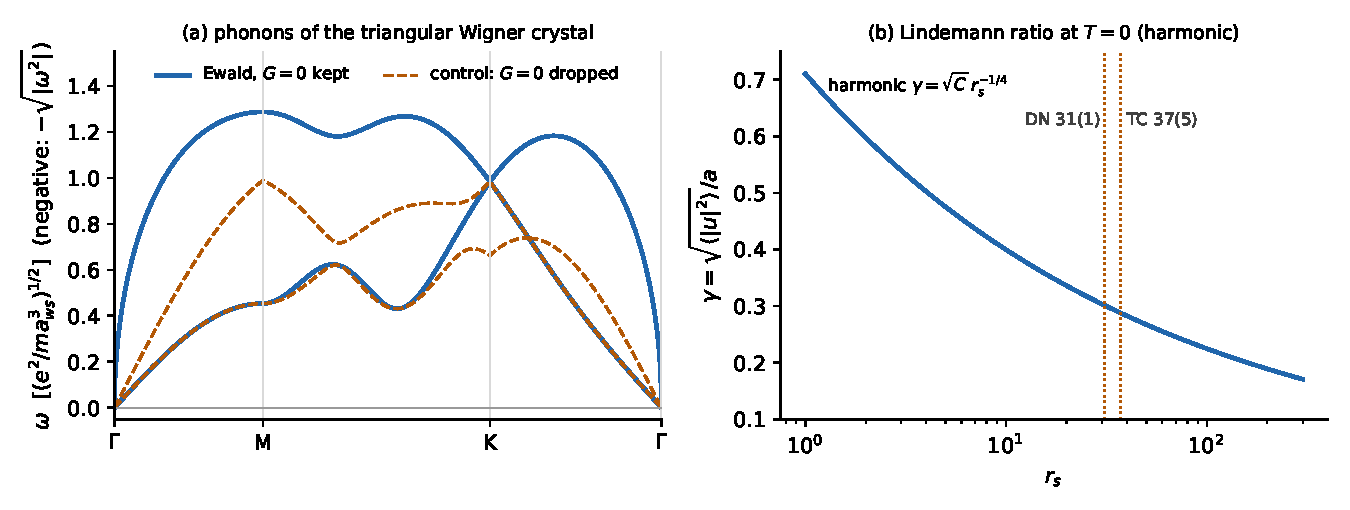
\includegraphics[width=\textwidth]{figures_v2/qm_phonons_lindemann.pdf}
\caption{(a) Phonon dispersion of the triangular Wigner crystal along $\Gamma$--M--K--$\Gamma$ in reduced units
(solid), and the negative control N2 with the $q=-k$ reciprocal term dropped (dashed): the longitudinal plasmon
$\omega_L\propto\sqrt{|k|}$ disappears. The imaginary modes of N2 lie off this path (6.4\% of the $48\times48$
grid). (b) Harmonic Lindemann ratio $\gamma=\sqrt C\,r_s^{-1/4}$, $C=0.504946$, with the QMC crystallisation
densities of Drummond--Needs (DN, $r_s=31(1)$) and Tanatar--Ceperley (TC, $37(5)$)~\cite{dn2009,tanatar}. Both panels
\tierX{} except the two QMC values \tierL. Produced by \texttt{code/quantum\_melting.py}.}\label{qm:fig}
\end{figure}

How to read it:
\begin{itemize}
\item \emph{Positive controls} \tierX. Changing the Ewald parameter from $\alpha=1$ to $0.6$ or $1.6$ changes $D(k)$ by
at most $1.6\times10^{-15}$: round-off. The trace sum rule agrees with the Ewald-free direct sum to the six printed
digits (the last digit of the third $k$ differs by one unit, the size of the neglected oscillating tail). The ratio
$\omega_L^2/|k|$ approaches $2=2\pi n$ in reduced units, with an error proportional to $|k|$. The transverse sound
speed is $c_T=0.371837$ in units of $(e^2/ma_{\rm ws})^{1/2}$.
\item \emph{Convergence in the grid} \tierX. The average of $\sum\omega$ converges with observed order $p=2.52$ and is
changes by $2.2\times10^{-7}$ between $m=192$ and $m=384$. The average of $\sum1/\omega$ converges only with order
$p=1.01$, as expected from the $1/|k|$ singularity of the integrand: halving the grid spacing halves the error. Its
value at $m=384$ ($3.66090$) is still $7\times10^{-4}$ relative below the Richardson extrapolation ($3.663483$), and
we use the extrapolated value. A student who stopped at $m=24$ would have made an error of $1.2\%$; a grid that
\emph{contained} $k=0$ would have divided by zero.
\item \emph{Positive control against the literature.} Our zero-point coefficient is $c_{\rm zp}=0.813686$ Hartree
($1.627372$ Rydberg) \tierX. Drummond and Needs quote, from Bonsall and Maradudin, the analytically determined
coefficients $c_1=-1.106103$ and $c_{3/2}=0.814$ of the low-density expansion
$E=c_1r_s^{-1}+c_{3/2}r_s^{-3/2}+\dots$, in Hartree atomic units, the second being ``the quasiharmonic zero-point
phonon energy''~\cite{dn2009,bm} \tierL. Our value agrees with $0.814$ within the rounding of a three-digit number
($0.814\pm0.0005$). (The first coefficient is the Madelung constant $\eta=-1.106102587$ used by the Rust crate of
Chapter~3, rounded.) We did not read Bonsall and Maradudin's paper itself; the comparison is with the value as
quoted by Drummond and Needs.
\item \emph{The zero-point displacement} \tierX: $C_{\rm ws}=1.831741$, i.e.\
$\langle|u|^2\rangle=1.831741\,a_{\rm ws}^2\,r_s^{-1/2}$, and $C=0.504946$ in \eqref{qm:eq-C}.
\item \emph{Negative control N1} \tierX. The classical average $\langle\sum\omega^{-2}\rangle$ grows by the same amount,
$\approx2.51$, at every doubling of $m$: logarithmic growth. Its slope per unit $\ln m$ is $3.61701$, against
$1/(2c_T^2)=3.61630$ predicted by Proposition~\ref{qm:prop-finite} (in reduced units $n=1/\pi$, and $\ln N=2\ln m$).
The quantum averages in the same table converge; the classical one does not, and it fails in exactly the predicted
way.
\item \emph{Negative control N2} \tierX. With the $q=-k$ term dropped, $6.4\%$ of the grid points have an imaginary
frequency ($\min\omega^2=-0.0417$), and at $|k|=10^{-3}$ both branches are of order $10^{-7}$ instead of
$\omega_L^2\approx2\times10^{-3}$: the plasmon is gone (Figure~\ref{qm:fig}a, dashed). Such a crystal would be
unstable, and its zero-point quantities meaningless. The correct calculation has no imaginary frequency on any grid
used (the averages of $1/\omega$ would otherwise be complex, and the script would fail).
\end{itemize}

%---------------------------------------------------------------------
\subsection{The Lindemann criterion}\label{qm:sec-lindemann}

The Lindemann criterion is a rule of thumb for melting (named after F.~A.~Lindemann; we cite no source for its
history): a crystal melts when the root mean square displacement of its
particles reaches a fixed fraction $\gamma_c$ of the spacing. It is a heuristic, not a theorem: melting is a
competition of free energies (or, at $T=0$, of ground-state energies) between two phases, and the rule looks only at
one of them \tierC. Its value lies in turning a hard question (where is the phase boundary?) into an easy one (how big
are the vibrations?), at the price of one empirical constant.

\paragraph{Conventions matter.} In this section $\gamma^2=\langle|u|^2\rangle/a^2$, where $|u|^2$ sums \emph{both}
Cartesian components and $a$ is the \emph{nearest-neighbour} spacing. Other authors use one component (a factor
$\sqrt2$ in $\gamma$), $a_{\rm ws}$ instead of $a$ (a factor $1.9046$), or relative displacements of neighbours
(below). A value of $\gamma_c$ can only be carried from one paper to another after converting conventions.

\paragraph{The quantum Lindemann density.} With \eqref{qm:eq-C}, $\gamma=\sqrt C\,r_s^{-1/4}$, and setting
$\gamma=\gamma_c$ gives the melting density
\begin{equation}\label{qm:eq-rsstar}
r_s^\ast=\Bigl(\frac{C}{\gamma_c^2}\Bigr)^{2}=\frac{C^2}{\gamma_c^4}\qquad(C=0.504946).
\end{equation}
\tierC{} for the criterion, \tierX{} for $C$. The fourth power is the lesson. To first order a relative error
$\delta$ in $\gamma_c$ becomes $4\delta$ in $r_s^\ast$; exactly, $\gamma_c\to0.9\gamma_c$ multiplies $r_s^\ast$ by
$0.9^{-4}=1.52$ and $\gamma_c\to1.1\gamma_c$ by $1.1^{-4}=0.68$. A ten-percent uncertainty in a rule of thumb becomes
a factor-of-two uncertainty in the prediction. The script prints:
\begin{center}
\begin{tabular}{c|ccccccccc}
\toprule
$\gamma_c$ & 0.20 & 0.22 & 0.24 & 0.26 & 0.28 & 0.30 & 0.33 & 0.36 & 0.40\\
$r_s^\ast$ & 159.4 & 108.8 & 76.9 & 55.8 & 41.5 & 31.5 & 21.5 & 15.2 & 10.0\\
\bottomrule
\end{tabular}
\end{center}

\paragraph{Comparison with quantum Monte Carlo.} The crystallisation density of the two-dimensional electron gas has
been computed by quantum Monte Carlo. Tanatar and Ceperley found crystallisation at $r_s=37\pm5$~\cite{tanatar}, and
Drummond and Needs, with smaller error bars, found a transition from a paramagnetic fluid to an antiferromagnetic
triangular Wigner crystal at $r_s=31(1)$~\cite{dn2009} \tierL. The harmonic Lindemann ratio at these densities is
$\gamma=0.301$ ($r_s=31$) and $0.288$ ($r_s=37$) \tierX.

Read this the right way round. We did not \emph{predict} $r_s^\ast\approx31$: we have no independent value of
$\gamma_c$, and the row $\gamma_c=0.30\mapsto r_s^\ast=31.5$ matches Drummond--Needs because $0.30$ is, by construction,
the harmonic $\gamma$ at $r_s=31$. What the calculation provides is a \emph{calibration}: in the conventions above,
the harmonic Lindemann ratio at the QMC transition is about $0.29$--$0.30$ \tierX/\tierC. Three caveats \tierC:
\begin{enumerate}
\item The harmonic approximation underestimates $\langle|u|^2\rangle$ near melting, where anharmonic terms are no
longer small; the true $\gamma$ at $r_s=31$ is presumably larger.
\item The QMC transition is a crossing of two ground-state energies (a first-order transition), not an instability of
the crystal. The crystal exists, as a metastable state, on both sides of it.
\item The criterion knows nothing about spin, exchange, or the fluid; Drummond and Needs' transition is to an
antiferromagnetic crystal, a distinction no Lindemann argument can make.
\end{enumerate}

\paragraph{At $T>0$: relative displacements.} Proposition~\ref{qm:prop-finite} shows that at $T>0$ the classical
$\langle|u|^2\rangle$ of a two-dimensional crystal is infinite in the thermodynamic limit, so the ratio $\gamma$ is
infinite at every temperature and the criterion in this form cannot be used. The remedy is to measure the displacement of a
particle \emph{relative to its neighbour}, $u_{R+\delta}-u_R$ with $|\delta|=a$, which stays finite: the factor
$1-\cos k\cdot\delta\sim(k\cdot\delta)^2$ removes the divergence at $k=0$. This modified criterion has been
proposed for two-dimensional melting~\cite{bedanov} \tierL. The script computes it in the harmonic approximation.
With the classical coupling $\Gamma=e^2/(a_{\rm ws}k_BT)$,
\begin{equation}\label{qm:eq-rel}
\gamma_{\rm rel}^2:=\frac{\langle|u_{R+\delta}-u_R|^2\rangle}{a^2}
=\frac{2}{\Gamma}\,\frac{\langle\sum_\lambda(1-\cos k\cdot\delta)\,\omega_{\lambda}^{-2}\rangle_{\rm BZ}}{(a/a_{\rm ws})^2}
=\frac{2.978022}{\Gamma}\quad\text{(classical)},
\end{equation}
and $\gamma_{\rm rel}^2=0.787282\,r_s^{-1/2}$ for the zero-point motion at $T=0$ \tierX. The classical average
converges (it changes by $5\times10^{-5}$ between $m=192$ and $m=384$; the quantum one by $1.5\times10^{-7}$). Grimes and
Adams observed the freezing of electrons on helium at $\Gamma=137\pm15$, where their $\Gamma$ is ``a measure of the
ratio of potential energy to kinetic energy per electron''~\cite{grimes} \tierL. If, as is customary, that $\Gamma$ is
$e^2(\pi n)^{1/2}/k_BT$ --- which is our $e^2/(a_{\rm ws}k_BT)$ --- then \eqref{qm:eq-rel} gives the harmonic relative
Lindemann ratio at the observed classical melting point, $\gamma_{\rm rel}=0.147$ \tierX; the identification of
conventions is our assumption \tierC. The quantum value at $r_s=31$ is $\gamma_{\rm rel}=0.376$. The two numbers
differ by a factor of $2.5$; this is a warning, not a contradiction. Classical melting in two dimensions is driven by
defects (dislocations), quantum melting competes with a Fermi liquid, and a single ``universal'' Lindemann constant
covering both is not to be expected \tierC.

%---------------------------------------------------------------------
\subsection{Transition-metal dichalcogenides and exciton fluids}\label{qm:sec-tmd}

This book has not discussed these systems before; they are a new application, in the spirit of
Section~\ref{sec:ch4-other}.

\paragraph{Electrons in TMD layers.} Monolayers of transition-metal dichalcogenides (such as MoSe$_2$ and WSe$_2$)
are two-dimensional semiconductors. In a material, the Bohr radius of \eqref{qm:eq-rs} is replaced by the effective
Bohr radius $a_B^\ast=\varepsilon\hbar^2/(m^\ast e^2)$, with the band mass $m^\ast$ and the dielectric constant
$\varepsilon$ of the surroundings; the potential-to-kinetic ratio is $r_s=a_{\rm ws}/a_B^\ast$. A heavy band mass and
weak screening make $a_B^\ast$ small and $r_s$ large at densities that gates can reach \tierC. %%TMD%%

\paragraph{Interlayer excitons are dipoles.} In a heterobilayer, an electron in one layer and a hole in the other,
a distance $d$ apart, bind into an \emph{interlayer exciton}: a boson carrying an electric dipole $p=ed$
perpendicular to the layers. Model each exciton as a charge $+e$ in one plane and $-e$ directly below it in a
parallel plane at distance $d$. Two excitons at in-plane distance $r$ then interact through two like-charge pairs at
distance $r$ and two unlike pairs at distance $\sqrt{r^2+d^2}$:
\begin{equation}\label{qm:eq-exciton}
U(r)=e^2\Bigl(\frac2r-\frac2{\sqrt{r^2+d^2}}\Bigr)\;=\;\frac{e^2d^2}{r^3}+O\Bigl(\frac{d^4}{r^5}\Bigr)\quad(r\gg d)
\end{equation}
(Exercise~\ref{qm:ex-dipole}). This is the same structure as the image-charge interaction of electrons on helium
(Section~\ref{sec:ch4-plasmas}, with $2d$ there in place of $d$ here). Two facts follow.

\begin{proposition}[the two-plane exciton potential is admissible]\label{qm:prop-cm}
For every $d>0$, $h(t)=\frac2{\sqrt t}-\frac2{\sqrt{t+d^2}}$ (that is, $U$ as a function of $t=r^2$, with $e=1$)
satisfies \lean{AdmissiblePotential}: it is $C^\infty$ on $(0,\infty)$, nonnegative, and $(-1)^rh^{(r)}(t)\ge0$ for all
$r\ge0$, $t>0$.
\end{proposition}
\begin{humanproof}
\tierC{} (complete, but not in Lean). The direct route: $\frac{d^r}{dt^r}(t+c)^{-1/2}=(-1)^r\frac{(2r-1)!!}{2^r}(t+c)^{-1/2-r}$
for $c\ge0$, with $(-1)!!=1$. Hence
\[
(-1)^rh^{(r)}(t)=\frac{2\,(2r-1)!!}{2^r}\Bigl(t^{-1/2-r}-(t+d^2)^{-1/2-r}\Bigr)>0,
\]
because $x\mapsto x^{-1/2-r}$ is decreasing and $t<t+d^2$. The case $r=0$ is the nonnegativity, and smoothness is
clear. A second proof shows \emph{why}, in the language of Chapter~1: from
$t^{-1/2}=\pi^{-1/2}\int_0^\infty\alpha^{-1/2}e^{-\alpha t}\,d\alpha$,
\[
h(t)=\frac{2}{\sqrt\pi}\int_0^\infty e^{-\alpha t}\,\alpha^{-1/2}\bigl(1-e^{-\alpha d^2}\bigr)\,d\alpha ,
\]
a Gaussian mixture (in $r$) with a nonnegative weight. The weight vanishes like $\alpha^{1/2}$ at $\alpha=0$, so the
mixture contains no constant, and the warning about constants in Chapter~1 does not apply.
\end{humanproof}

The last block of the script output checks the proposition independently, at 40 significant digits, for $r=0,\dots,10$
and $t$ on a logarithmic grid from $10^{-3}$ to $10^3$: no negative value for $d^2\in\{0.1,1,10\}$, while the
Lennard-Jones control $4(t^{-6}-t^{-3})$ fails already at $r=0$ (it is negative for $t>1$) \tierX. The check can
fail, and it does when it should; it is a sanity check of the algebra, not a proof.

Consequently \tierA{} conditional on Proposition~\ref{qm:prop-cm} (which is \tierC): for every density $\rho>0$, the
kernel-checked \lean{universal_any_density} (Chapter~2, D2) applies to $h$, and the triangular lattice at density
$\rho$ has the least lower energy among all locally finite configurations of density $\rho$, in this model. Its lattice
energy is finite, because $h(t)\le d^2t^{-3/2}$ for large $t$ and $s=3>2$. This is a statement about \emph{classical,
static} dipoles. The scope is narrow:
\begin{itemize}
\item It concerns the two-plane point-charge model \eqref{qm:eq-exciton} only. In real TMD heterostructures the
in-layer interaction is screened by the layers themselves (a Rytova--Keldysh-type form), which is a different function;
we have not checked whether it is admissible \tierC.
\item Excitons are composite quantum bosons. The classical minimiser tells us around which arrangement they would
vibrate if they crystallised, not whether they do.
\end{itemize}

\paragraph{Where would excitons crystallise?} For the tail $e^2d^2/r^3$, \eqref{qm:eq-ratio} with $s=3$ and
$C=e^2d^2$ gives a potential-to-kinetic ratio $\propto(m_Xe^2d^2/\hbar^2)\,n^{1/2}$, with $m_X$ the exciton mass:
dipolar excitons crystallise, if at all, at \emph{high} density \tierC. %%DIPOLE%%
But the dipolar form holds only when the spacing is large compared with $d$. Push the density so high that the spacing
falls below $d$, and \eqref{qm:eq-exciton} becomes $U\approx e^2(2/r-2/d)$: an $s=1$ law plus a constant, which by
the same scaling crystallises only at \emph{low} density. Any exciton crystal therefore lives in a window of
densities, bounded above roughly where the spacing reaches $d$ --- and, physically, also by the density at which
excitons overlap and dissociate into an electron--hole plasma \tierC. Whether that window is non-empty for given
materials is a quantitative question this section does not answer.

\begin{warnbox}[: what this section does and does not claim]
Kernel-checked here: nothing new. Proved by hand (Tier~C): the exciton model potential is admissible, so the
classical theorem applies to it at every density. Computed (Tier~X): the harmonic phonons, zero-point energy and
zero-point displacement of the two-dimensional Wigner crystal, with the controls above. From the literature (Tier~L):
the QMC crystallisation densities, the Grimes--Adams $\Gamma$, the observations in TMDs. Heuristic (Tier~C): the
scaling argument and every use of the Lindemann criterion. The quantum melting of a triangular crystal is outside the
theorem.
\end{warnbox}

\subsection*{Exercises for Section~\ref{qm:sec}}

\begin{exercise}\label{qm:ex-fermi}
For a spin-$\frac12$ Fermi gas in two dimensions with both spin states equally occupied, show that $k_F^2=2\pi n$ and
$E_F=\pi\hbar^2n/m$. Show that the mean kinetic energy per particle is $E_F/2$, and that, in Hartree atomic units,
it equals $1/(2r_s^2)$ \emph{Hartree}, i.e.\ $1/r_s^2$ \emph{Rydberg}. Compare its $r_s$ dependence with that of the
Madelung energy $c_1/r_s$ and of $E_{\rm zp}$ in \eqref{qm:eq-laws}, and explain why $E_{\rm zp}\propto r_s^{-3/2}$
lies between the two.
\end{exercise}

\begin{exercise}\label{qm:ex-einstein}
\emph{An Einstein model.} Replace the phonon spectrum by a single frequency: one particle moves in the field of all
the others held fixed. Show that the restoring matrix is $\sum_{R\ne0}\Phi(R)=\Psi(0)$ and that, by the trace sum
rule, its trace is $\sum_{R\ne0}R^{-3}$ (in units $e=m=1$, $a_{\rm ws}=1$). Using the six-fold symmetry, show that
$\Psi(0)$ is a multiple of the identity and find its Einstein frequency $\omega_E$. Compute
$\sum_{R\ne0}R^{-3}$ numerically (direct sum with a tail correction, as in check P2). Then compare
$c_{\rm zp}^{E}=\omega_E$ and $C^E_{\rm ws}=1/\omega_E$ with the phonon values $0.813686$ and $1.831741$. Which
quantity does the Einstein model get better, and why does it overestimate the zero-point energy? (Hint: Jensen's
inequality, since $\omega_E^2$ is the average of $\omega_\lambda^2$.)
\end{exercise}

\begin{exercise}\label{qm:ex-dipole}
Derive \eqref{qm:eq-exciton} and its expansion for $r\gg d$, including the next term. Then: (a) show that $U(r)$ is
strictly decreasing; (b) using Proposition~\ref{qm:prop-cm}, write $U$ as a Gaussian mixture and identify the mixing
weight; (c) show that the image-charge potential $\frac1r-\frac1{\sqrt{r^2+4d^2}}$ of Section~\ref{sec:ch4-plasmas} is
admissible by the same argument; (d) show that the potential $\frac1r+\frac1{\sqrt{r^2+d^2}}$ (two like charges in
each pair of planes) is also admissible, and explain why it is nevertheless outside the finite-energy class.
\end{exercise}

\begin{exercise}\label{qm:ex-convergence}
Modify \texttt{code/quantum\_melting.py}: (a) use an \emph{unshifted} grid that contains $k=0$ and explain the error
you get; (b) exclude $k=0$ from the unshifted grid and compare the convergence of $\langle\sum1/\omega\rangle$ with the
shifted grid; (c) treat the region $|k|<k_0$ analytically, using $\omega_T\simeq c_T|k|$ and $\omega_L^2\simeq2|k|$, and
show that this improves the order of convergence. Report your actual output, and state whether your extrapolated $C$
agrees with $0.504946$.
\end{exercise}
